\documentclass[tikz,border=2pt]{standalone}
\usepackage[T1]{fontenc}
\usepackage{lmodern}
\usepackage{amsmath}
\usepackage[table]{xcolor}
\usepackage{tikz}
\usetikzlibrary{arrows.meta,calc,positioning}

\definecolor{paletteGreen}{HTML}{2A6F62}
\definecolor{paletteOrange}{HTML}{D96C3D}

\begin{document}
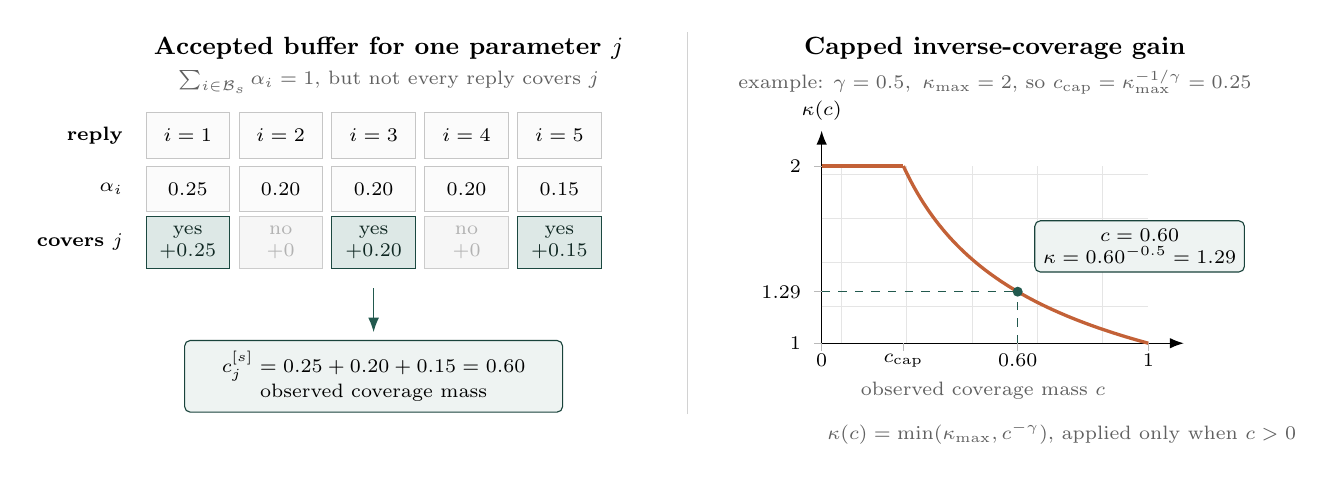
\begin{tikzpicture}[
  font=\scriptsize,
  >=Latex,
  cell/.style={minimum width=1.06cm, minimum height=0.58cm, draw=gray!45, line width=0.3pt, align=center},
  covered/.style={cell, fill=paletteGreen!16, draw=paletteGreen!65!black, text=paletteGreen!35!black},
  missing/.style={cell, fill=gray!7, draw=gray!40, text=gray!60},
  note/.style={align=center, text=gray!75!black},
  paneltitle/.style={font=\small\bfseries, align=center}
]
  \node[paneltitle] at (2.55,3.85) {Accepted buffer for one parameter \(j\)};
  \node[note] at (2.55,3.42) {\(\sum_{i\in\mathcal{B}_s}\alpha_i=1\), but not every reply covers \(j\)};

  \node[anchor=east, font=\scriptsize\bfseries] at (-0.70,2.74) {reply};
  \node[anchor=east, font=\scriptsize\bfseries] at (-0.70,2.06) {\(\alpha_i\)};
  \node[anchor=east, font=\scriptsize\bfseries] at (-0.70,1.38) {covers \(j\)};

  \foreach \x/\name/\weight/\state in {
    0/{1}/0.25/yes,
    1.18/{2}/0.20/no,
    2.36/{3}/0.20/yes,
    3.54/{4}/0.20/no,
    4.72/{5}/0.15/yes
  } {
    \node[cell, fill=gray!3] at (\x,2.74) {\(i=\name\)};
    \node[cell, fill=gray!3] at (\x,2.06) {\(\weight\)};
  }
  \node[covered] at (0,1.38) {yes\\\(+0.25\)};
  \node[missing] at (1.18,1.38) {no\\\(+0\)};
  \node[covered] at (2.36,1.38) {yes\\\(+0.20\)};
  \node[missing] at (3.54,1.38) {no\\\(+0\)};
  \node[covered] at (4.72,1.38) {yes\\\(+0.15\)};

  \draw[->, line width=0.5pt, paletteGreen!80!black]
    (2.36,0.80) -- (2.36,0.24);
  \node[
    rounded corners=2pt,
    draw=paletteGreen!60!black,
    fill=paletteGreen!8,
    align=center,
    inner sep=4pt,
    minimum width=4.8cm
  ] at (2.36,-0.32)
    {\(c_j^{[s]}=0.25+0.20+0.15=0.60\)\\observed coverage mass};

  \draw[gray!35, line width=0.4pt] (6.35,-0.80) -- (6.35,4.05);

  \node[paneltitle] at (10.25,3.85) {Capped inverse-coverage gain};
  \node[note] at (10.25,3.42) {example: \(\gamma=0.5,\ \kappa_{\max}=2\), so \(c_{\mathrm{cap}}=\kappa_{\max}^{-1/\gamma}=0.25\)};

  \coordinate (origin) at (8.05,0.10);
  \draw[->, line width=0.45pt] (origin) -- (12.65,0.10);
  \draw[->, line width=0.45pt] (origin) -- (8.05,2.80)
    node[above, font=\scriptsize] {\(\kappa(c)\)};

  \foreach \cx/\lab in {0/{0},0.25/{\(c_{\mathrm{cap}}\)},0.60/{0.60},1/{1}} {
    \draw[gray!55] ({8.05+4.15*\cx},0.10) -- ({8.05+4.15*\cx},0.00);
    \node[below, font=\scriptsize] at ({8.05+4.15*\cx},0.09) {\lab};
  }
  \foreach \ky/\lab in {1/{1},1.29/{1.29},2/{2}} {
    \draw[gray!55] (8.05,{0.10+2.25*(\ky-1)}) -- (7.95,{0.10+2.25*(\ky-1)});
    \node[left, font=\scriptsize] at (7.91,{0.10+2.25*(\ky-1)}) {\lab};
  }

  \draw[gray!20, line width=0.25pt] (8.05,0.10) grid[xstep=0.83, ystep=0.5625] (12.20,2.35);
  \draw[paletteOrange!90!black, very thick]
    plot[domain=0:0.25, samples=2] ({8.05+4.15*\x},{0.10+2.25});
  \draw[paletteOrange!90!black, very thick]
    plot[domain=0.25:1, samples=70] ({8.05+4.15*\x},{0.10+2.25*(1/sqrt(\x)-1)});

  \draw[dashed, paletteGreen!80!black]
    ({8.05+4.15*0.60},0.10) -- ({8.05+4.15*0.60},{0.10+2.25*(1/sqrt(0.60)-1)});
  \draw[dashed, paletteGreen!80!black]
    (8.05,{0.10+2.25*(1/sqrt(0.60)-1)}) -- ({8.05+4.15*0.60},{0.10+2.25*(1/sqrt(0.60)-1)});
  \fill[paletteGreen!80!black] ({8.05+4.15*0.60},{0.10+2.25*(1/sqrt(0.60)-1)}) circle (1.8pt);
  \node[
    rounded corners=2pt,
    draw=paletteGreen!60!black,
    fill=paletteGreen!8,
    align=center,
    inner sep=3pt,
    anchor=west
  ] at (10.75,1.33) {\(c=0.60\)\\\(\kappa=0.60^{-0.5}=1.29\)};

  \node[align=center, text=gray!75!black] at (10.10,-0.50) {observed coverage mass \(c\)};
  \node[anchor=north west, align=left, text=gray!75!black] at (8.00,-0.78)
    {\(\kappa(c)=\min(\kappa_{\max},c^{-\gamma})\), applied only when \(c>0\)};
\end{tikzpicture}
\end{document}
